%!TEX root =../../../course-notes.tex
% ^ leave for LaTeXTools build functionality

\begin{applicationActivities}



\begin{definition}
  A subset of a vector space is called a \term{subspace} if it is
  a vector space on its own.

  \vspace{1em}

  For example, the span of these two vectors forms a planar subspace
  inside of the larger vector space \(\IR^3\).

  \begin{center}
  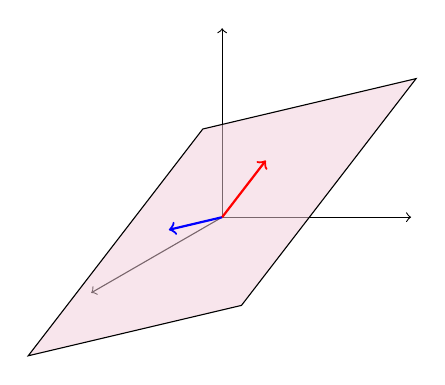
\begin{tikzpicture}[x={(210:0.8cm)}, y={(0:1cm)}, z={(90:1cm)},scale=0.4]
    \draw[->] (0,0,0) -- (6,0,0);
    \draw[->] (0,0,0) -- (0,6,0);
    \draw[->] (0,0,0) -- (0,0,6);
    \draw[fill=purple!20,fill opacity=0.5]
      (-2,-2,2) -- (6,-2,-2) -- (2,2,-2) -- (-6,2,2) -- (-2,-2,2);
    \draw[thick,blue,->] (0,0,0) -- (1,-1,0);
    \draw[thick,red,->] (0,0,0) -- (-2,0,1);
  \end{tikzpicture}
  \end{center}
\end{definition}



\begin{fact}
  Any sub\textbf{set} \(S\) of a vector space \(V\) satisfies the eight
  vector space properties automatically, since it is a collection of known
  vectors.

  \vspace{1em}

  However, to verify that it's a sub\textbf{space}, we need to check that
  addition and multiplication still make sense using only vectors from \(S\).
  So we need to check two things:

  \begin{itemize}
  \item The set is \textbf{closed under addition}: for any \(\vec{x},\vec{y} \in S\), the sum \(\vec{x}+\vec{y}\) is also in \(S\).
  \item The set is \textbf{closed under scalar multiplication}: for any \(\vec{x} \in S\) and scalar \(c \in \IR\), the product \(c\vec{x}\) is also in \(S\).
\end{itemize}
\end{fact}

\begin{activity}{15}
Let \(S=\setBuilder{\begin{bmatrix} x \\ y \\ z \end{bmatrix}}{ x+2y+z=0}\).

\begin{subactivity}
  Let \(\vec{v}=\begin{bmatrix} x \\ y \\ z \end{bmatrix}\) and
  \(\vec{w} = \begin{bmatrix} a \\ b \\ c \end{bmatrix} \) be vectors in \(S\),
  so \(x+2y+z=0\) and \(a+2b+c=0\). Show that
  \(\vec v+\vec w = \begin{bmatrix} x+a \\ y+b \\ z+c \end{bmatrix}\)
  also belongs to \(S\) by verifying that \((x+a)+2(y+b)+(z+c)=0\).
\end{subactivity}
\begin{subactivity}
  Let \(\vec{v}=\begin{bmatrix} x \\ y \\ z \end{bmatrix}\in S\), so
  \(x+2y+z=0\). Show that \(c\vec v\) also belongs to \(S\) for any
  \(c\in\IR\).
\end{subactivity}
\begin{subactivity}
  Is \(S\) is a subspace of \(\IR^3\)?
\end{subactivity}
\end{activity}

\begin{activity}{10}
Let \(S=\setBuilder{\begin{bmatrix} x \\ y \\ z \end{bmatrix}}{ x+2y+z=4}\).
Choose a vector
\(\vec v=\begin{bmatrix} \unknown\\\unknown\\\unknown \end{bmatrix}\) in \(S\)
and a real number \(c=\unknown\), and show that \(c\vec v\) isn't in \(S\).
Is \(S\) a subspace of \(\IR^3\)?
\end{activity}

\begin{remark}
Since \(0\) is a scalar and \(0\vec{v}=\vec{z}\) for any vector \(\vec{v}\), a
set that is closed under scalar multiplication must contain the zero vector
\(\vec{z}\) for that vector space.

\vspace{1em}

Put another way, an easy way to check that a subset isn't a subspace is to
show it doesn't contain \(\vec 0\).
\end{remark}

\begin{activity}{10}
  Consider these two subsets of \(\IR^4\):
  \[
    S=
    \setBuilder{ \begin{bmatrix}a\\b\\-b\\-a\end{bmatrix}}{a,b\text{ are real numbers}}
    \hspace{3em}
    T=
    \setBuilder{ \begin{bmatrix}a\\b\\b-1\\a-1\end{bmatrix}}{a,b\text{ are real numbers}}
  \]
  \begin{subactivity}
  Which set is not a subspace of \(\IR^4\)?
  \end{subactivity}
  \begin{subactivity}
  Is the set of polynomials
  \[S=
    \setBuilder{ ax^3+bx^2+(b-1)x+(a-1)}{a,b\text{ are real numbers}}
  \]
  a subspace of \(\P^3\)?
\end{subactivity}
\end{activity}

\begin{activity}{10}
  Consider the subset \(A\) of \(\IR^2\) where at least one coordinate of
  each vector is \(0\).
  \begin{center}
    \begin{tikzpicture}[scale=0.25]
    \draw[thin,gray,<->] (-5,0) -- (5,0);
    \draw[thin,gray,<->] (0,-5) -- (0,5);
    \draw[thick,blue] (-4.8,0) -- (4.8,0);
    \draw[thick,blue] (0,-4.8) -- (0,4.8);
    \end{tikzpicture}
  \end{center}

This set contains \(\vec 0\), and
it's not hard to show that for every \(\vec v\) in \(A\) and scalar \(c\in\IR\),
\(c\vec v\) is also in \(A\). Is \(A\) a subspace of \(\IR^2\)? Why?

  \begin{instructorNote}
    Sketch the sum of two vectors on different axes to give a geometrical
    argument.
  \end{instructorNote}
\end{activity}

% \begin{activity}{10}
%   Prove that \(P=\setBuilder{ax^2+b}{a,b \in \IR}\) is a subspace
%   of the vector space of all degree-two polynomials by showing it is closed under addition and scalar multiplication.
% \end{activity}
%
% \begin{activity}{10}
% Let \(P=\setBuilder{x}{x\in\IR\text{ and }x>0}\) be the set of all positive
% real numbers.  Determine if \(P\) is a subspace of \(\IR\) or not.
% \end{activity}



\begin{activity}{5}
Let \(W\) be a subspace of a vector space \(V\).  How are \(\vspan W\) and \(W\) related?
\begin{enumerate}[(a)]
\item \(\vspan W\) is bigger than \(W\)
\item \(\vspan W\) is the same as \(W\)
\item \(\vspan W\) is smaller than \(W\)
\end{enumerate}
\end{activity}

\begin{fact}
  If \(S\) is any subset of a vector space \(V\), then
  since \(\vspan S\) collects all possible linear combinations,
  \(\vspan S\) is automatically a subspace of \(V\).

  \vspace{1em}

  In fact, \(\vspan S\) is always the smallest
  subspace of \(V\) that contains all the vectors in \(S\).
\end{fact}

\end{applicationActivities}
